\chapter{實驗 2：厚度極限測試與剪切鎖死評估}

\section{座標軸詳細物理意義說明}
在厚度敏感度與自鎖測試圖表中，座標軸的決定機制如下：
\begin{itemize}
\item \textbf{橫軸（X 軸）：板物理厚度 $\log_{10}(h)$} \\
此處的 $h$ 代表板的真實幾何厚度。圖表中數據點\textbf{由右向左}（從 $-1.0$ 降低至 $-5.0$），代表結構厚度呈幾何級數縮減，最左側的 $-5.0$ 點對應 $h = 1.0 \times 10^{-5}$ 的超薄板物理極限。
\item \textbf{縱軸（Y 軸）：誤差對數 $\log_{10}(\text{Error})$} \\
代表在固定 $17 \times 17$ 網格下，各流派在不同厚度條件下的絕對誤差高低。本圖表不評估收斂率斜率，而是觀測線條在薄板極限下的數值穩定波動趨勢。
\end{itemize}

\section{數值結果對比與鎖死分析}
圖~\ref{fig:exp2_omega}、圖~\ref{fig:exp2_w}~與圖~\ref{fig:exp2_phi}~展示了結構在厚度變更考驗下的誤差反應。

\begin{figure}[h]
\centering
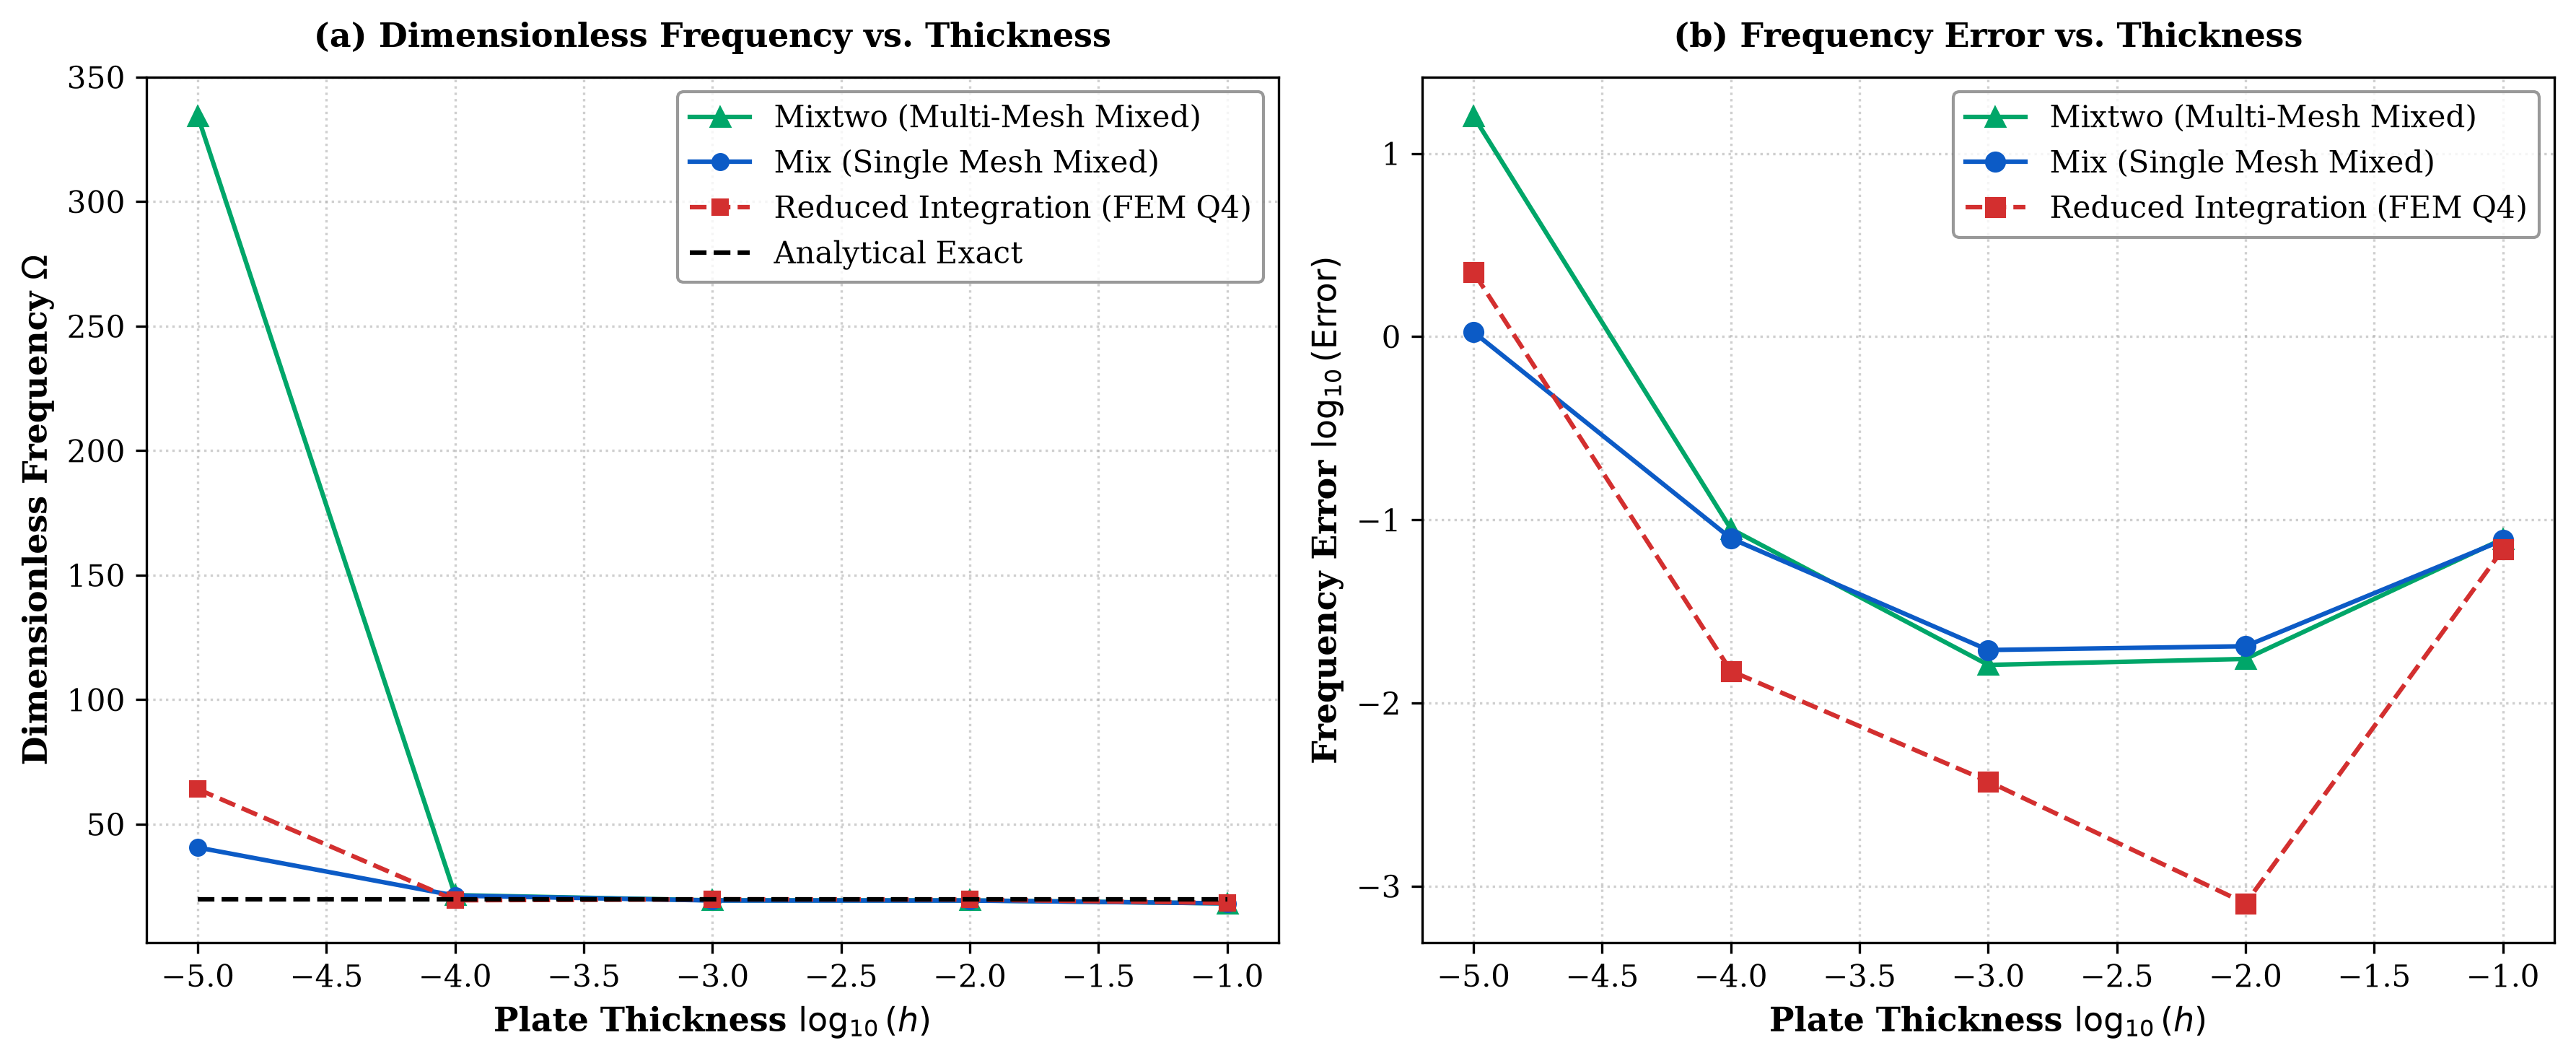
\includegraphics[width=0.8\textwidth]{vibration_thickness_omega_analysis.png}
\caption{固有頻率與相對誤差隨板幾何厚度縮減之響應曲線}
\label{fig:exp2_omega}
\end{figure}

依據數據結果，傳統有限元（FEM Q4）在厚度變薄的過程中發生了嚴重的數值剛度自鎖。當 $\log_{10}(h)$ 降至 $-5.0$ 時，傳統有限元的頻率相對誤差對數劇烈反彈飆升至 \textbf{0.35116}，數值精度徹底失效。與之相對，混合法體系（Mix 與 Mixtwo）隨厚度變薄其誤差線條始終壓制在低位區間，Mix 在 $-5.0$ 處的誤差對數僅為 0.02453，成功免疫了剪切鎖死現象。

\begin{figure}[h]
\centering
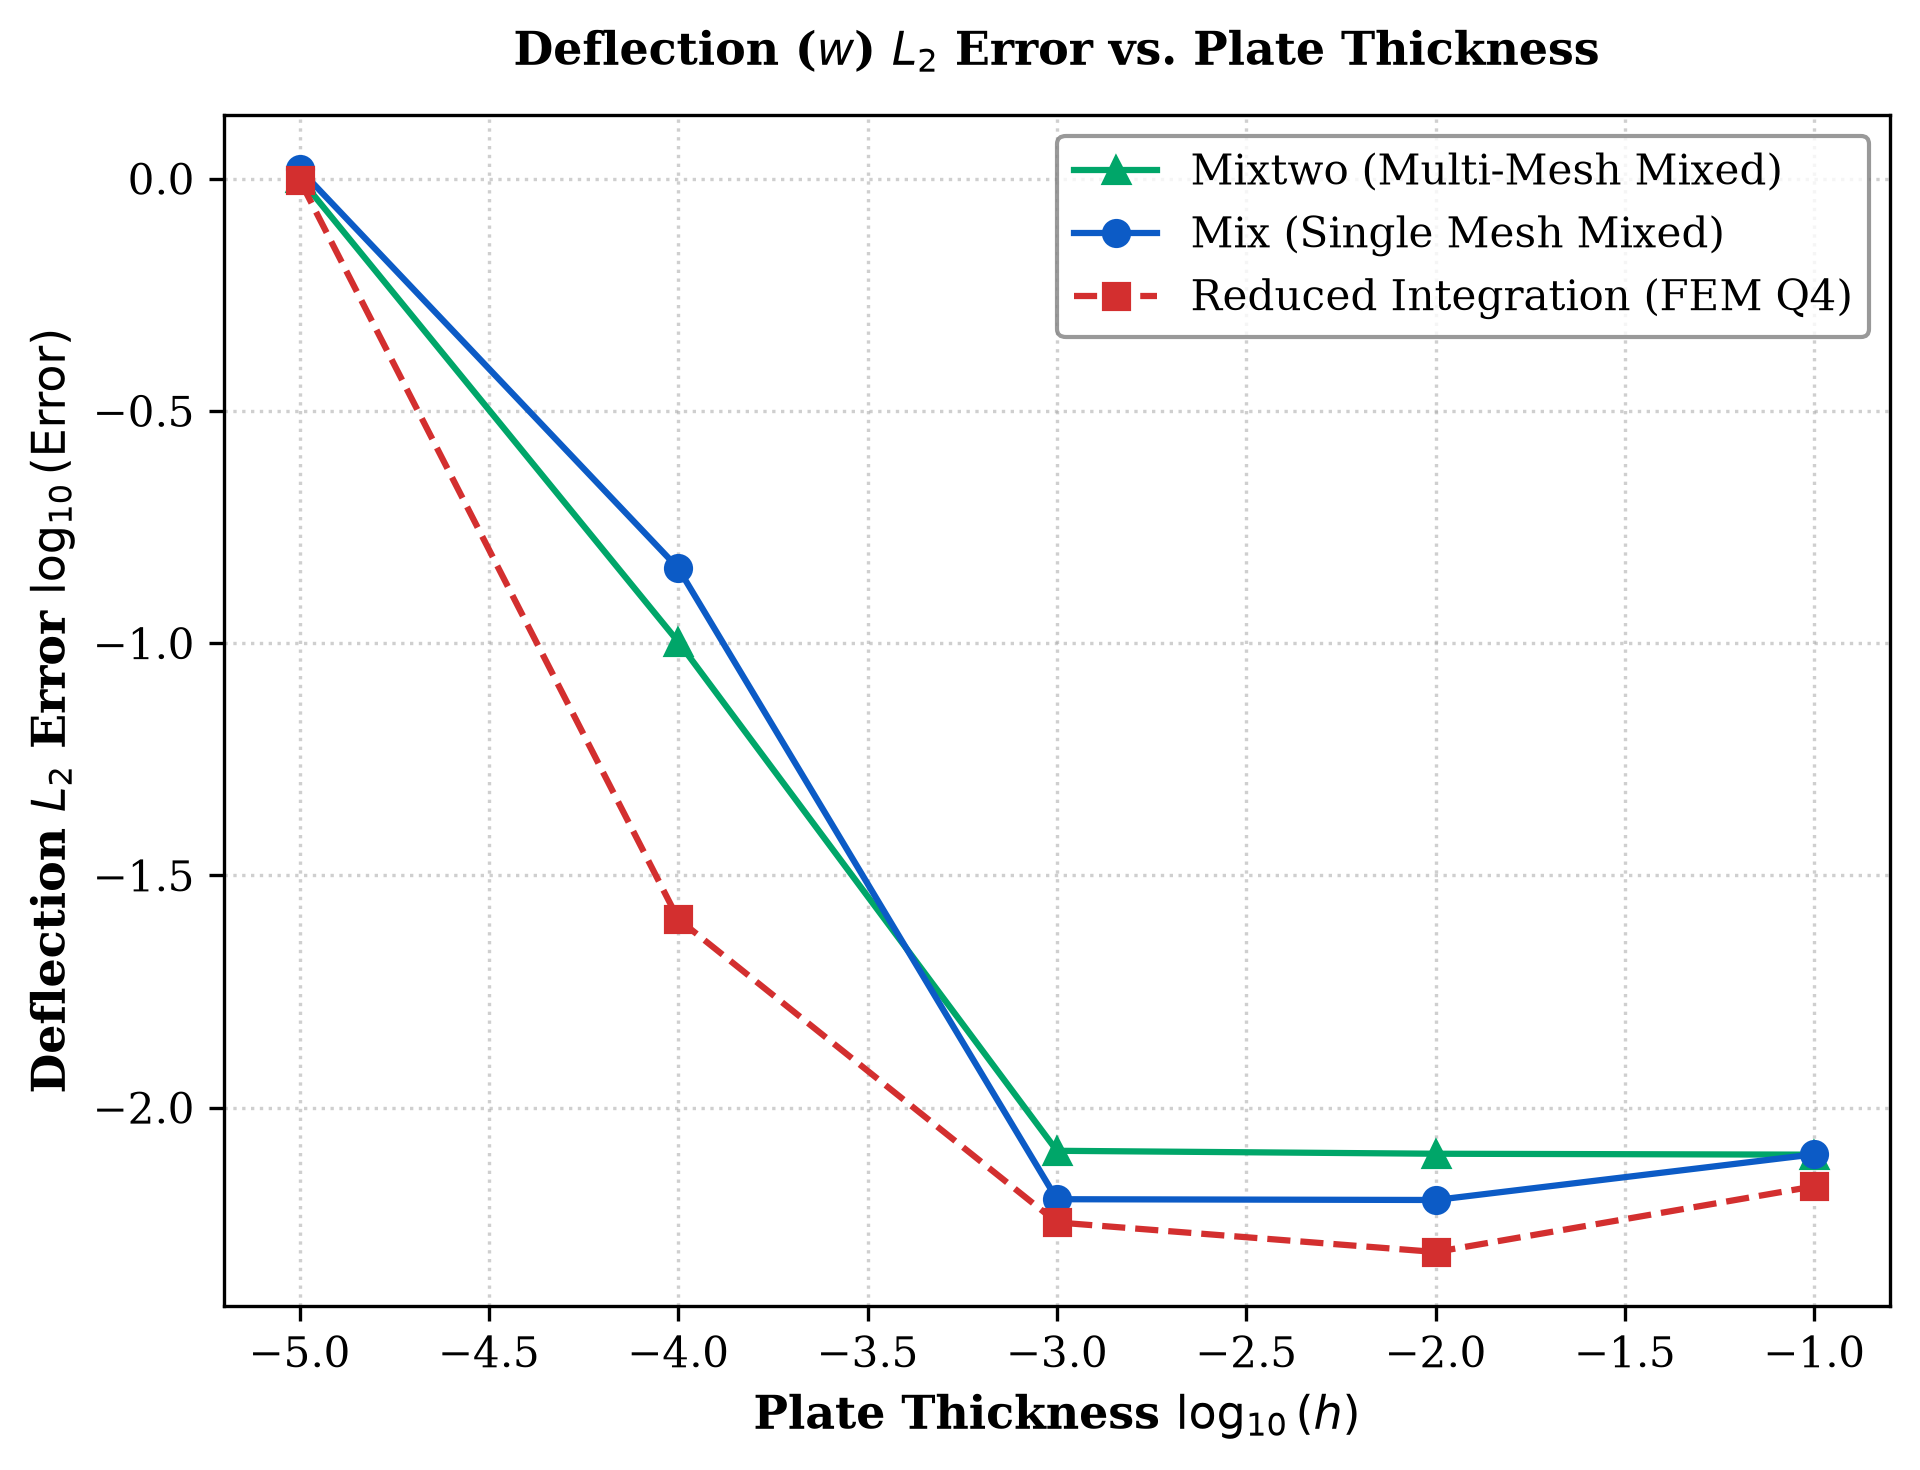
\includegraphics[width=0.6\textwidth]{vibration_thickness_w_convergence.png}
\caption{位移場（$w$）$L_2$ 誤差隨幾何厚度縮減之響應折線}
\label{fig:exp2_w}
\end{figure}

在位移場全域殘差測試中（圖~\ref{fig:exp2_w}），傳統有限元（紅線）在薄板極限區間無法展現幾何收斂，殘差直接在高位死線平盤橫變。而藍線（Mix）與綠線（Mixtwo）在全幾何跨度下，其位移 $L_2$ 殘差不升反降，全線維持在低水平區間穩定延伸，未受數值鎖死干擾。

\begin{figure}[h]
\centering
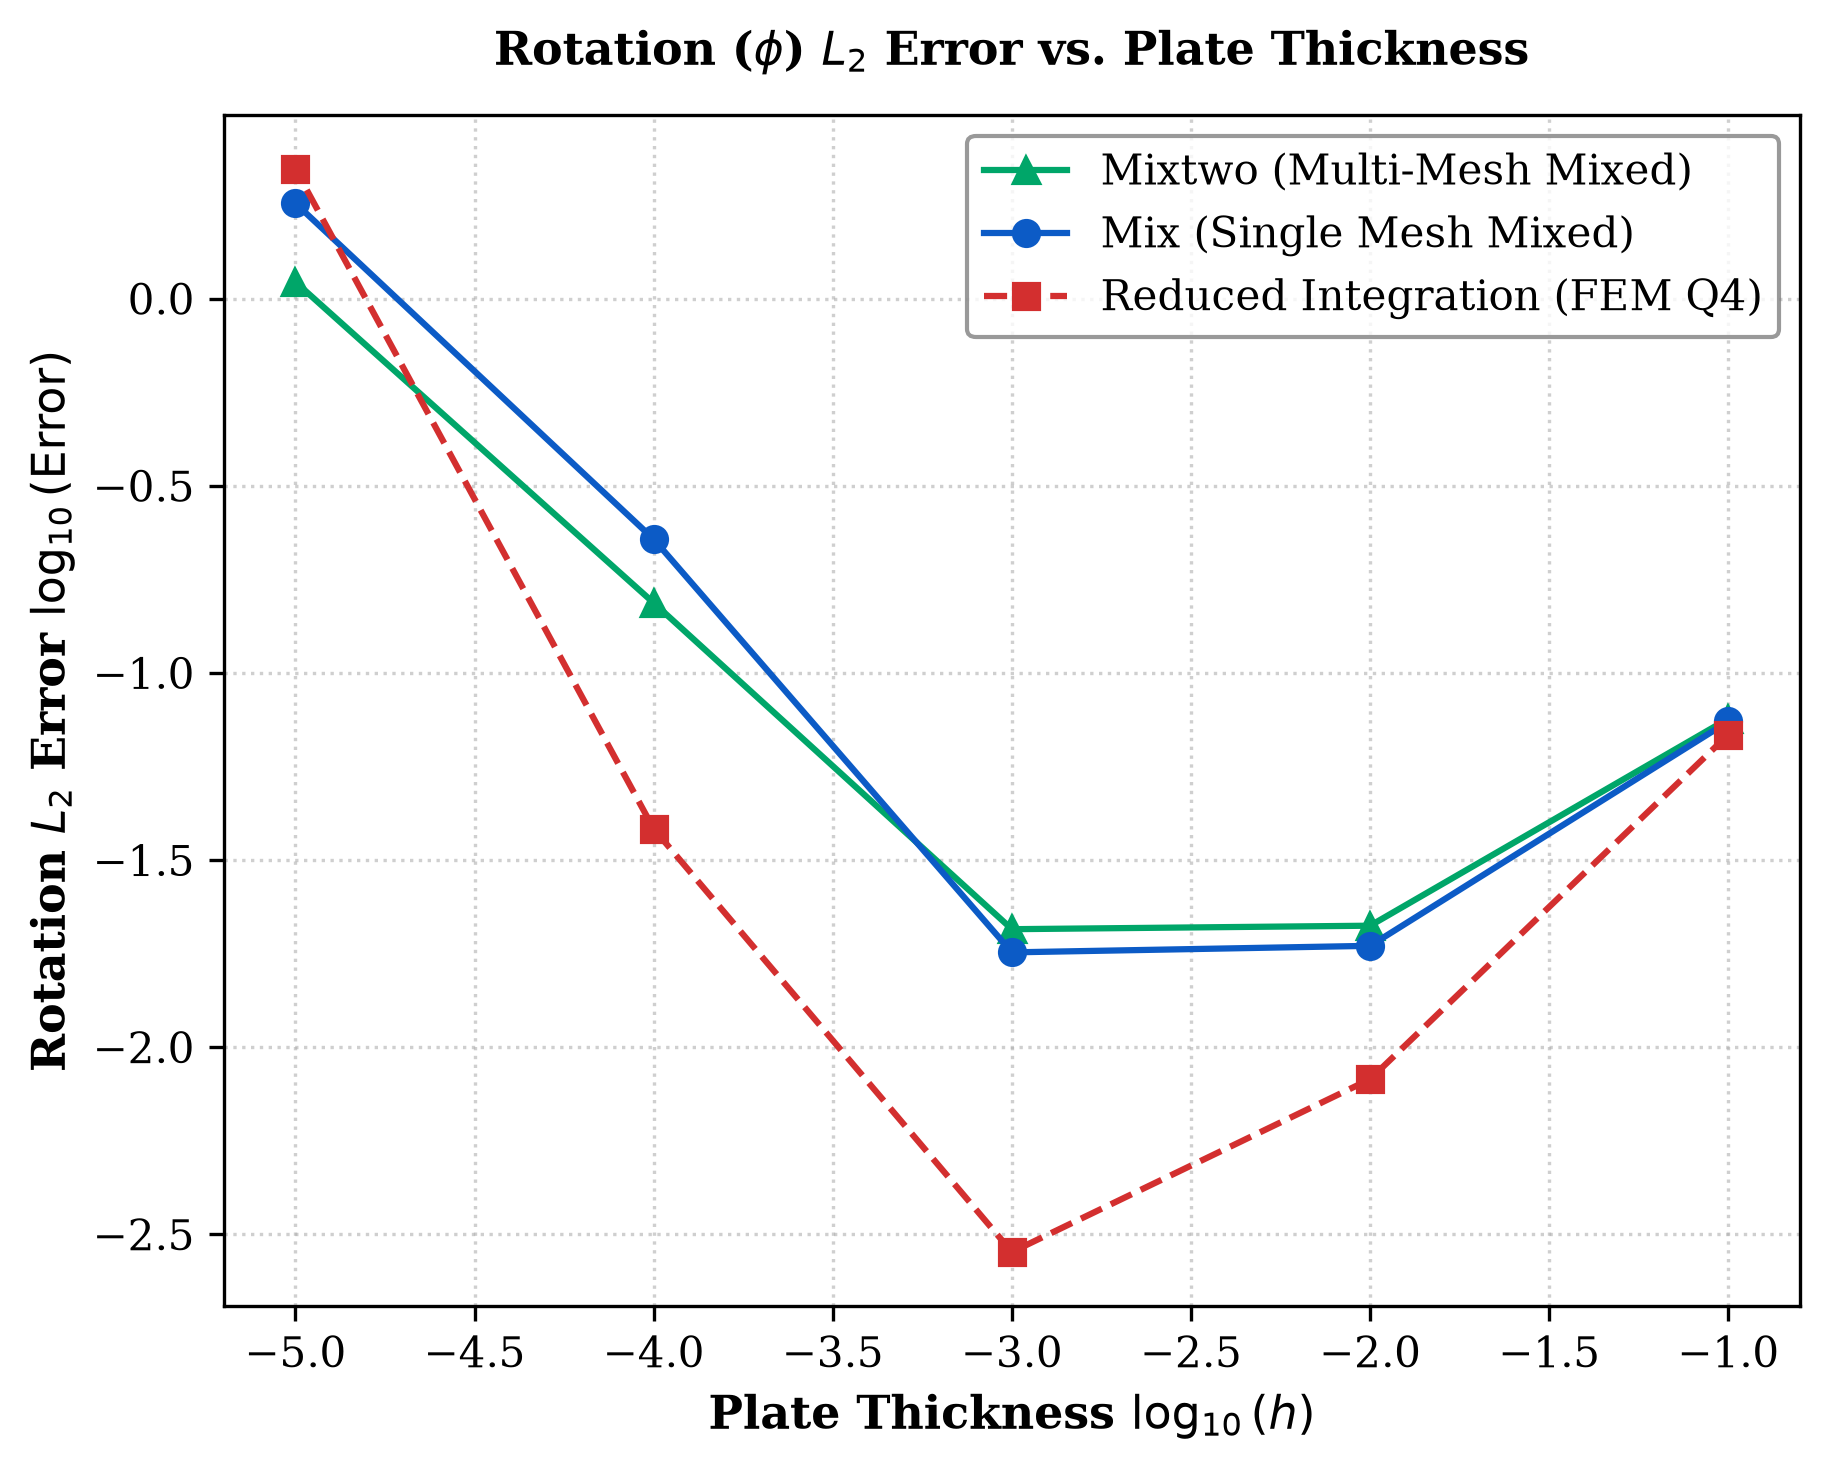
\includegraphics[width=0.6\textwidth]{vibration_thickness_phi_convergence.png}
\caption{轉角場（$\phi$）$L_2$ 誤差隨幾何厚度縮減之響應折線}
\label{fig:exp2_phi}
\end{figure}

如圖~\ref{fig:exp2_phi}~所示，轉角場的幾何殘差展現出與位移場高度一致的力學規律。傳統有限元（紅線）在超薄區域誤差擴大，而基於無網格重構核與多場混合變分的 Mix 與 Mixtwo 流派，在全域厚度範圍內皆表現出極佳的數值穩定性與力學正確性。